%!TEX root=../../root.tex

\section{Lezione 3}
\subsection{Operazioni tra linguaggi regolari}
Siano $A_1$ e $A_2$ due automi a stati finiti possiamo definire un automa $A$ che accetti il risultato di una certa operazione tra il linguaggio di $A_1:$ e il linguaggio di $A_2$.
Per ogni operazione binaria possiamo definire l'automa come segue:
\[
	A = (Q_1 \times Q_2, \Sigma, \delta, q_0, F)
\]
\[
	\delta = (Q_1 \times Q_2) \times \Sigma \to Q_1 \times Q_2
\]
Definita come segue:
\[
	\delta ((q_1, q_2), a) = (\delta_1 (q_1, a), \delta_2 (q_2, a) )
\]
\[
	q_0 = (q_0^1, q_0^2)
\]
Possiamo definire anche $\delta^{\star}$:
\[
	\delta^{\star} ( (q_1, q_2), x) = (\delta_1^{\star} (q_1, x), \delta_2^{\star} (q_2, x))
\]
Ora definiamo F per le due operazioni binarie.
\subparagraph{Unione di linguaggi regolari}
\[
	\exists A \in DFA \; L(A)=L(A_1) \cup L(A_2)
\]
\[
	Q = \{ (q_1, q_2) | q_1 \in Q_1 \land q_2 \in Q_2 \}
\]
\[
	F = (Q_1 \times F_2) \cup (F_1 \times Q_2)
\]
\subparagraph{Intersezione di linguaggi regolari} 
\[
	\exists A \in DFA \; L(A)=L(A_1) \cap L(A_2)
\]
\[
	Q = \{ (q_1, q_2) | q_1 \in Q_1 \land q_2 \in Q_2 \}
\]
\[
	F = F_1 \times F_2 
\]
\subparagraph{Complemento di un linguaggio regolare} Definiamo separatamente il complemento di un linguaggio regolare.
\[
	L \in REG \Rightarrow \exists A \in DFA t.c. L(A) = L
\] 
\[
	A = (Q, \Sigma, \delta, q_0, F)
\] 
\[
	A^c = (Q, \Sigma, \delta, q_0, Q-F)
\]
\[
	L(A) \in REG \Leftrightarrow L^c(A) \in REG
\]

\subsection{Problemi di riduzioni, da automi a grafi}
Per rispondere ad alcune domande sugli automi \`e comodo ridurre il problema ad un problema sui grafi.\newline
\begin{description}
	\item \emph{Esempio 1}: dato un automa $A$ vogliamo sapere se $L(A)$ \`e finito, questo problema si pu\`o ridurre alla ricerca di un ciclo in un grafo. Per applicare l'algoritmo di ricerca dei cicli dobbiamo avere un \emph{automa ridotto}, ossia un grafo che rappresenti l'automa solamente con stati che appartengono a cammini da $q_0$ ad un qualsiasi stato in $F$ o da un qualsiasi stato in $F$ a $q_0$. 

	\item \emph{Esempio 2}: dato un automa $A$ vogliamo sapere se $L(A)=\emptyset$, questo problema si pu\`o ridurre alla ricerca di un percorso da $q_0$ ad un qualsiasi stato in $F$. Se non esistono cammini da $q_0$ ad un qualsiasi stato in $F$ allora $L(A)=\emptyset$.
\end{description}
Questi due problemi verranno discussi in dettaglio nella lezione 4.

\subsection{Operazioni su parole}
\subparagraph{Concatenazione} 
\begin{description}
	\item $x, y \in \Sigma^{\star} \Rightarrow xy \in \Sigma^{\star}$
	\item elemento neutro: $\varepsilon$, $x \varepsilon = x = \varepsilon x$
\end{description}
\subparagraph{Potenza}
\begin{description}
	\item $x \in \Sigma^{\star} \Rightarrow x^n = x. . .x $(x concatenata n volte con se stessa) $\in \Sigma^{\star}$
	\item elemento neutro: $1$, $x^1 = x$
	\item elemento cancellatore: $0$, $x^0 = \varepsilon$
\end{description}
\subsection{Operazioni su linguaggi}
\subparagraph{Concatenazione}
\begin{description}
	\item $L,L' \in REG \Rightarrow LL'=\{x | x \in \Sigma^{\star} \land \exists y \in L, z \in L' \land x=yz \}$
	\item elemento neutro: $\{\varepsilon\}$, $L \{\varepsilon\} = L =  \{\varepsilon\} L$
	\item elemento cancellatore: $\emptyset$, $L \emptyset = \emptyset =  \emptyset L$
\end{description}
\subparagraph{Potenza}
\begin{description}
	\item $L \in REG \Rightarrow L^n = \{ x^n | x \in L \land n \geq 0 \}$
	\item elemento neutro: $1$, $L^1 = L$
	\item elemento cancellatore: $0$, $L^0 = \{\varepsilon$\}
\end{description}
\subparagraph{Estensione o stella di Kleene}
\begin{description}
	\item $L^{\star} = \bigcup_{i \geq 0} L^i$
	\item Questa operazione fu introdotta nel 1976 da Robin e Scott.
\end{description}

\subsection{Automi non deterministici}
\subparagraph{In generale}
Un automa a stati finiti non deterministico, in breve NFA, \`e un automa in cui esistono passi di calcolo non \`e univocamente determinati.\newline
Immaginiamo di avere una macchina per il seguente automa:
\begin{figure}[H]
	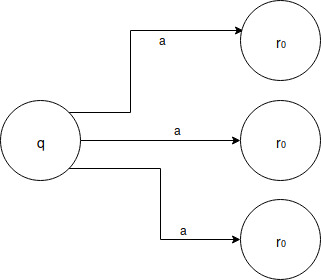
\includegraphics[scale=0.5]{nfa0}
\end{figure}
Possiamo immaginare la macchina eseguire i passi che corrispondono ad una sequenza di input e per ogni passo non univocamente determinato abbiamo delle macchine equivalenti che proseguono la computazione parallelamente per ogni possibile scelta di passo successivo.\newline
Introduciamo ora il concetto di \emph{configurazione}, sostanzialmente \`e un' estensione del concetto di stato e consiste nella coppia $(q, x)$ dove $q$ \`e uno stato dell'automa e $x$ \`e la parola in input allo stato $q$.\newline
Utilizzando le configurazioni possiamo rappresentare l'albero della computazione. Notare che nel caso di DFA abbiamo un albero degenere.
\subparagraph{Primi esempi}
\begin{description}
	\item \emph{Esempio 1}: $L =  \{x1y | x \in \Sigma^{\star} \land y \in \Sigma^2\}$, ossia tutte le stringhe che hanno $1$ come terzultimo simbolo.\newline
	Automa:
	\begin{figure}[H]
		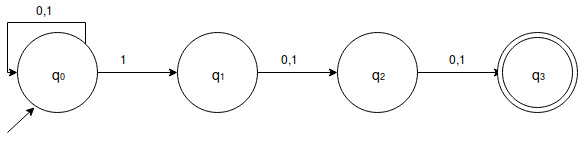
\includegraphics[scale=0.7]{nfa1}
	\end{figure}
	Albero della computazione:
	\begin{figure}[H]
		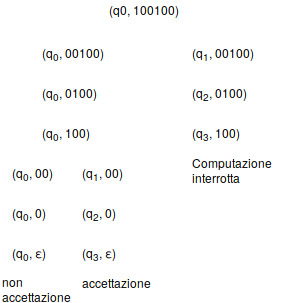
\includegraphics[scale=0.7]{nfa1alb}
	\end{figure}
	\item \emph{Esempio 2}: $L = \{ x0010 | x \in \Sigma^{\star}\} \cup \{ x100 | x \in \Sigma^{\star}\}$
	Automa:
	\begin{figure}[H]
		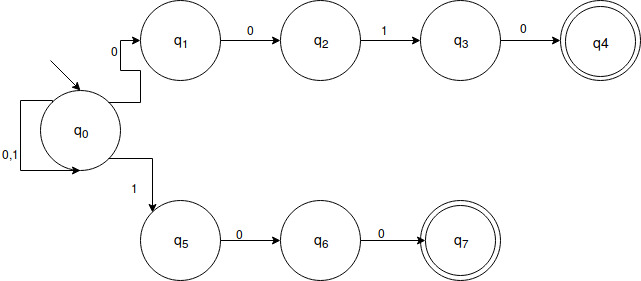
\includegraphics[scale=0.7]{nfa2}
	\end{figure}
\end{description}
\subsection{Dimostrazioni extra}
\subparagraph{Dimostrazione 1}

\[
	\delta^{\star} ( (q_1, q_2), x) = (\delta_1^{\star} (q_1, x), \delta_2^{\star} (q_2, x))
\]
Proviamo per induzione la precedente uguaglianza:\newline
Ricordiamo che la definizione di $\delta^{\star}$ \`e 
\begin{description}
	\item $\delta^{\star}(q, \varepsilon) = q \forall q \in Q$ 
	\item $\delta^{\star}(q, xa) = \delta(\delta^{\star}(q, x), a) \forall q \in Q, x \in \Sigma^{\star}, a \in \Sigma$
\end{description}
\begin{description}
	\item \emph{Passo base}: $x = \varepsilon$ \newline
	$\delta^{\star} ( (q_1, q_2), \varepsilon) = (q_1, q_2)$ per definizione di $\delta^{\star}$  ma $(q_1, q_2) = ( \delta(q_1, \varepsilon), \delta(q_2, \varepsilon))$
	\item \emph{Passo induttivo}: Supponiamo che l'uguaglianza valga per tutte le parole lunghe $n$, $(|x|=n, x \in \Sigma^{\star})$, e proviamo che valga per le parole lunghe $n+1$, $(xa, a \in \Sigma)$.
	\begin{description}
		\item $\delta^{\star} ((q_1, q_2), xa) = \delta ( \delta^{\star}((q_1, q_2),x), a)$ per definizione di $\Sigma^{\star}$
		\item $\delta ( ( \delta^{\star}((q_1, q_2),x), a) = \delta (( \delta_1^{\star}(q_1, x),\delta_2^{\star}(q_2,x)), a)$ per ipotesi induttiva
		\item $\delta ( (\delta_1^{\star}(q_1, x),\delta_2^{\star}(q_2,x)), a) = ( \delta_1 (\delta_1^{\star}(q_1, x),a), \delta_2(\delta_2^{\star}(q_2,x),a))$ per definizione di $\delta$
		\item $( \delta_1 (\delta_1^{\star}(q_1, x),a), \delta_2(\delta_2^{\star}(q_2,x),a)) = ( \delta_1^{\star}(q_1, xa), \delta_2^{\star}(q_2,xa))$ per definizione di $\delta^{\star}$ $\Box$
	\end{description}

\end{description}
\subparagraph{Dimostrazione 2}
Dati due automi $A_1 = (Q_1, \Sigma, \delta_1, q^1_0, F_1)$ con $L_1=L(A_1)$ e $A_2 = (Q_2, \Sigma, \delta_2, q^2_0, F_2)$ con $L_2=L(A_2)$ esiste $A = (Q = Q_1 \times Q_2, \Sigma, \delta, q_0, F = Q_1 \times F_2 \cup F_1 \times Q_2)$ tale che $L(A) = L(A_1) \cup L(A_2)$. Vogliamo dimostrare che:
\[
	x \in L(A) \Leftrightarrow x \in L(A_1) \lor x \in L(A_2)
\]
\[
	x \in L(A) \Leftrightarrow
\]
\[
	 \delta^{\star} ((q^1_0, q^2_0), x) \in F \Leftrightarrow
\]
\[	
	 (\delta_1^{\star}(q^1_0, x),\delta_1^{\star}(q^2_0, x)) \in F = Q_1 \times F_2 \cup F_1 \times Q_2) \Leftrightarrow 
\]
\[	 
	 \delta_1^{\star}(q^1_0, x) \in F_1 \lor \delta_1^{\star}(q^2_0, x) \in F_2 \Leftrightarrow 
\]
\[	 
	 x \in L(A_1) \lor x \in L(A_2) \Box
\]
